%versi 2 (8-10-2016)
\chapter{Landasan Teori}
\label{chap:teori}

Pengelompokan dokumen berkaitan erat dengan dua bidang ilmu dalam informatika. Pe-ngelompokan dalam informatika merupakan bagian dari bidang pembelajaran mesin. Dalam pembelajaran mesin, terdapat dua jenis pengelompokan, yaitu \textit{clustering} dan \textit{classification}. \textit{Clustering} merupakan salah satu jenis pembelajaran tak terarah (\textit{unsupervised learning}) karena setiap elemen dikelompokkan berdasarkan karakteristik dari elemen tersebut. Sedangkan \textit{classification} merupakan jenis pembelajaran terarah (\textit{supervised learning}) karena setiap elemen dikelompokkan berdasarkan label yang telah ditentukan sebelumnya. Pada penelitian ini, jenis pengelompokan yang akan digunakan adalah \textit{clustering}.

Domain masalah dalam penelitian ini adalah dokumen sehingga sangat erat kaitannya dengan bidang temu kembali informasi (\textit{information retrieval}). Sebelum dapat diolah lebih lanjut, dokumen-dokumen yang telah ada harus diolah sehingga menjadi suatu bentuk dengan nilai informasi yang dapat dimanipulasi oleh komputer. Biasanya dokumen akan direpresentasikan ke dalam bentuk vektor yang disebut dengan model ruang vektor.

\section{Temu Kembali Informasi}
\label{sec:tki}
Temu kembali informasi adalah bidang ilmu yang berurusan dengan representasi, penyimpanan, pengolahan, dan akses terhadap informasi.\cite{baeza1999modern} Pada penelitian ini, temu kembali informasi memiliki peran untuk mengubah dokumen yang semula berbentuk teks menjadi sesuatu yang memiliki nilai informasi agar nantinya bisa diproses lebih lanjut (dalam kasus ini dengan pengelompokan dokumen).

Dalam penelitian ini, temu kembali informasi digunakan untuk merepresentasikan dokumen ke dalam model ruang vektor agar bisa dilakukan pengelompokan. Tahap pertama yang dilakukan adalah membentuk kosa kata (\textit{vocabulary}) yang berisi seluruh istilah berbeda yang ada di setiap dokumen yang akan diindeks. Kemudian, untuk setiap dokumen akan dibentuk suatu indeks yang terdiri dari pasangan antara istilah di dokumen tersebut dan jumlah kemunculannya (\textit{term-document incidence matrix}). Tabel \ref{tbl:term-doc} merupakan contoh dari \textit{term-document incidence matrix} dengan baris pada tabel menunjukkan istilah (\textit{term}) dan kolom menunjukkan nama dokumen. Sel bernilai $1$ apabila dokumen mengandung term tertentu dan $0$ jika tidak.

Selanjutnya, setiap jumlah kemunculan suatu istilah dalam sebuah dokumen akan diubah menjadi suatu bobot tertentu berdasarkan teknik pemodelannya. Dalam penelitian ini, digunakan 2 teknik pembobotan yaitu bobot frekuensi dan bobot tf-idf.

\subsection{Bobot frekuensi}
Bobot frekuensi merupakan teknik pembobotan yang sangat sederhana karena bobotnya merupakan jumlah kemunculan istilah tersebut dalam dokumen. Bobot frekuensi dapat digambarkan dengan Persamaan \ref{eq:bobot}
\begin{equation}
\label{eq:bobot}
w_i=tf_i
\end{equation}
dengan $w_i$ merupakan bobot istilah ke-$i$ dan $tf_i$ merupakan frekuensi kemunculan istilah ke-$i$ pada dokumen.

\begin{table}[h]
\label{tbl:term-doc}
\centering
\begin{tabular}{lccccccc}
& \begin{tabular}[c]{@{}c@{}}Anthony\\ and \\ Cleopatra\end{tabular} & \begin{tabular}[c]{@{}c@{}}Julius \\ Caesar\end{tabular} & \begin{tabular}[c]{@{}c@{}}The \\ Tempest\end{tabular} & Hamlet & Othello & Macbeth & ... \\
Anthony		& 1 & 1 & 0 & 0 & 0 & 1 & \\
Brutus 		& 1 & 1 & 0 & 1 & 0 & 0 & \\
Caesar 		& 1 & 1 & 0 & 1 & 1 & 1 & \\
Calpurnia 	& 0 & 1 & 0 & 0 & 0 & 0 & \\
Cleopatra 	& 1 & 0 & 0 & 0 & 0 & 0 & \\
mercy 		& 1 & 0 & 1 & 1 & 1 & 1 & \\
worser 		& 1 & 0 & 1 & 1 & 1 & 0 & \\
...  
\end{tabular}
\caption{\textit{Term-document incidence matrix}}
\end{table}

\subsection{Bobot TF-IDF}
Pada bobot frekuensi, bobot hanya dihitung berdasarkan kemunculan istilah dalam dokumen itu sendiri. Namun dalam bobot TF-IDF (\textit{term frequency-inverse document frequency}), bobot juga dihitung berdasarkan kemunculan istilah pada himpunan dokumen. Metode ini sangat populer digunakan oleh sistem rekomendasi berbasis teks.\cite{aizawa2003information} Rumus dari pembobotan menggunakan TF-IDF ditunjukkan oleh Persamaan \ref{eq:tf-idf} 
\begin{equation}
\label{eq:tf-idf}
w_i=tf_i \times log \frac{N}{N_i}
\end{equation}
dengan $w_i$ merupakan bobot istilah ke-$i$, $tf_i$ merupakan frekuensi kemunculan istilah ke-$i$ pada dokumen, $N$ menyatakan banyaknya anggota himpunan dokumen, dan $N_i$ menunjukkan frekuensi dokumen dari istilah ke-$i$ (banyaknya dokumen pada himpunan dokumen yang memuat istilah ke-$i$).

Berdasarkan rumus tersebut, maka dapat ditarik dua kesimpulan yaitu:
\begin{itemize}
\item Semakin sering suatu istilah muncul di suatu dokumen, maka semakin representatif istilah tersebut terhadap isi dokumen.
\item Semakin banyak dokumen yang memuat suatu istilah, maka nilai informasi istilah tersebut semakin kecil.
\end{itemize}

Metode penetapan bobot TF-IDF dianggap sebagai metode yang berkinerja baik karena mempertimbangkan frekuensi kemunculan istilah baik secara lokal (TF) maupun global (IDF).


\subsection{Model ruang vektor}
Model ruang vektor adalah representasi dari koleksi dokumen sebagai vektor dalam ruang vektor yang umum.\cite{schutze2008introduction} Model ruang vektor ini biasanya digunakan dalam sejumlah operasi pencarian informasi mulai dari penilaian dokumen pada \textit{query}, klasifikasi dokumen dan pengelompokan dokumen.

Dalam pengolahan model ruang vektor, dibutuhkan cara untuk menghitung kesamaan antara dua ruang vektor. Dalam pengelompokan dokumen, apabila kesamaan antara dua buah vektor semakin besar, maka peluang kedua vektor tersebut berada dalam sebuah kelompok yang sama akan semakin besar. Dalam penelitian ini, digunakan dua cara untuk menghitung kesamaan antara dua ruang vektor yaitu menggunakan Jarak Euclidean (\textit{Euclidean distance}) dan persamaan cosinus (\textit{cosine similarity}).

\subsubsection{Jarak Euclidean}
\label{sub:euclideanDist}
Jarak Euclidean atau biasa disebut jarak garis lurus merupakan metode paling banyak digunakan untuk menghitung jarak antara dua buah vektor. Secara umum, rumus dari Jarak Euclidean ditunjukkan oleh persamaan \ref{eq:euclidean}
\begin{equation}
\label{eq:euclidean}
d_{ij}=\sqrt{\sum_{v=1}^N (x_{vi}-x_{vj})^2}
\end{equation}
dengan $d_{ij}$ adalah jarak antara vektor ke-$i$ dengan vektor ke-$j$, $N$ adalah jumlah dimensi pada vektor, dan $x_{vi}$ adalah nilai dimensi ke-$v$ dari vektor ke-$i$.

\subsubsection{Persamaan Cosinus}
\label{sub:cosineDist}
Persamaan cosinus merupakan normalisasi hasil kali titik dengan panjang masing-masing vektor. Persamaan cosinus ditunjukkan dalam persamaan \ref{eq:cosine}
\begin{equation}
\label{eq:cosine}
s_{ij}=\frac{i\cdot j}{\parallel i \parallel \times \parallel j \parallel}
\end{equation}
dengan $s_{ij}$ adalah kesamaan antara vektor ke-$i$ dengan vektor ke-$j$, $i$ adalah vektor ke-$i$, dan $j$ adalah vektor ke-$j$. Persamaan ini menjelaskan bahwa semakin kecil sudut antara dua vektor, maka tingkat kemiripannya semakin besar.

\section{Pembelajaran Mesin}
Pembelajaran mesin merupakan sistem yang dapat beradaptasi dengan keadaan baru dan dapat mengenali pola \cite{russell2016artificial}. Sistem yang telah belajar akan meningkatkan kinerjanya pada tugas-tugas di masa yang akan datang setelah melakukan pengamatan tentang lingkungannya. 

\subsection{Pengelompokan}
Tugas pengelompokan (\textit{clustering}) merupakan salah satu bagian dari pembelajaran mesin. Pengelompokan terdiri dari dua jenis berdasarkan metode pembelajarannya. \textit{Classification} merupakan jenis pembelajaran terarah karena sudah diberikan label sejak awal, lalu dilakukan pengelompokan berdasarkan label untuk setiap kelompoknya. Sedangkan \textit{clustering} merupakan jenis pembelajaran tak terarah karena tidak diberikan label sejak awal sehingga pengelompokan dilakukan berdasarkan suatu kesamaan tertentu.

\subsubsection{K-Means}
K-means merupakan algoritma pengelompokan yang paling populer digunakan saat ini. algoritma ini membagi data ke dalam $K$ \textit{cluster}. Setiap \textit{cluster} direpresentasikan dengan titik tengahnya (\textit{centroid}). Setiap iterasi, titik tengah akan dihitung sebagai rata-rata dari semua titik data dari \textit{cluster} tersebut. Persamaaan \ref{eq:kmeans} merupakan persamaan untuk menghitung \textit{centroid}
\begin{equation}
\label{eq:kmeans}
\mu_i=\frac{1}{N_i}\sum_{q=1}^{N_i}x_q
\end{equation}
dengan $\mu_i$ merupakan \textit{centroid} ke-$i$, $N_i$ merupakan jumlah titik data pada \textit{cluster} ke-$i$, dan $x_q$ merupakan titik ke-$q$ pada \textit{cluster} ke-$i$.

\begin{algorithm} % enter the algorithm environment
\caption{K-Means} % give the algorithm a caption
\label{alg:kmeans} % and a label for \ref{} commands later in the document
\begin{flushleft}
	\textbf{Input:} $S$ (himpunan titik data), $K$ (Jumlah \textit{cluster})\\
	\textbf{Output:} himpunan \textit{cluster}
\end{flushleft}
\begin{algorithmic}[1] % enter the algorithmic environment
	\STATE Pilih $K$ titik data sebagai himpunan awal \textit{centroid}.
	\REPEAT 
		\STATE Bentuk $K$ \textit{cluster} dengan menempatkan setiap titik data ke \textit{cluster} dengan \textit{centroid} terdekat.
		\STATE Hitung ulang \textit{centroid} untuk setiap \textit{cluster}. 
	\UNTIL{\textit{Centroid} tidak berubah.}
\end{algorithmic}
\end{algorithm}

Algoritma K-means diawali dengan penentuan \textit{centroid} secara acak. Pada setiap iterasi, setiap data ditetapkan pada \textit{cluster} yang memiliki \textit{centroid} dengan jarak terdekat dari titik data tersebut, kemudian posisi \textit{centroid} dari setiap \textit{cluster} akan dihitung ulang dengan Persamaan \ref{eq:kmeans}. Iterasi akan terus diulang sampai posisi dari semua \textit{cluster} tidak berubah.

\section{Algoritma Genetika}
Algoritma genetika (GA) adalah suatu algoritma pencarian yang terinspirasi dari proses seleksi alam yang terjadi secara alami dalam proses evolusi. Ada beberapa istilah yang digunakan dalam algoritma genetika di antaranya kromosom, seleksi, persilangan, mutasi, dan fungsi \textit{fitness}.

\subsection{Kromosom}
\label{sub:chromosome}
Dalam GA, kromosom adalah himpunan parameter yang mendefinisikan suatu solusi yang diusulkan. Kromosom biasanya direpresentasikan sebagai string yang berisi kumpulan nilai (gen), meskipun berbagai struktur data lainnya juga digunakan.

\subsection{Seleksi}
\label{sub:selection}
Seleksi dalam algoritma genetika bertugas untuk memilih kromosom dari populasi untuk proses persilangan berdasarkan nilai \textit{fitness}. Salah satu teknik yang populer digunakan dalam seleksi adalah \textit{roulette-wheel selection} atau \textit{fitness proportional selection}. \textit{Roulette-wheel selection} memilih suatu individu dari populasi dengan probabilitas yang sebanding dengan nilai \textit{fitness} relatifnya. Hal ini serupa dengan sebuah diagram lingkaran pada gambar \ref{fig:pieChart} di mana setiap kromosom telah dialokasikan sebuah bagian pada diagram sesuai dengan nilai \textit{fitness} relatif. Semakin tinggi nilai \textit{fitness}, maka semakin besar bagian yang dialokasikan dan semakin besar kemungkinan kromosom tersebut akan terpilih dalam proses seleksi.

Dalam GA, proses seleksi akan memilih sejumlah induk yang cukup untuk reproduksi dan membentuk generasi selanjutnya. Dalam penelitian ini diterapkan strategi \textit{elitism} yaitu dengan langsung memindahkan individu dengan nilai \textit{fitness} terbesar ke generasi selanjutnya. Hal ini dilakukan untuk mencegah individu tersebut terhilang dari populasi dalam proses reproduksi.

\begin{figure}[h]
	\begin{center}
		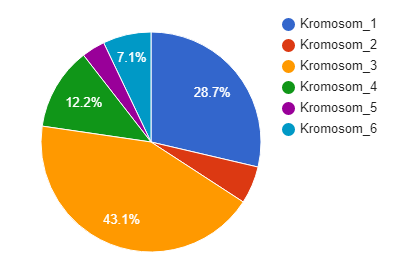
\includegraphics[scale=0.755]{pieChart}
		\caption{Diagram Lingkaran}
		\label{fig:pieChart}
	\end{center}
\end{figure}

\subsection{Persilangan}
\label{sub:crossover}
Persilangan adalah operasi genetik yang digunakan untuk menggabungkan informasi genetik dari dua induk untuk menghasilkan keturunan baru. Teknik persilangan yang digunakan dalam penelitian ini adalah \textit{Single-point crossover}. Dalam teknik ini, sebuah titik pada kedua induk dipilih untuk menjadi titik persilangan (\textit{crossover point}). Bit yang berada di sebelah kanan titik persilangan bertukar antara kedua kromosom induk seperti yang ditunjukkan pada Gambar \ref{fig:spcrossover}.

\begin{figure}[h]
	\begin{center}
		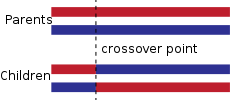
\includegraphics{OnePointCrossover}
		\caption{\textit{Single-point crossover}}
		\label{fig:spcrossover}
	\end{center}
\end{figure}

\subsection{Mutasi}
\label{sub:mutation}
Mutasi adalah suatu operator genetik yang digunakan untuk mempertahankan keragaman genetik dari satu generasi populasi dalam algoritma genetika. Mutasi mengubah satu atau beberapa nilai dalam gen. Mutasi terjadi berdasarkan probabilitas mutasi yang sudah ditentukan sebelumnya. Probabilitas ini seharusnya bernilai kecil, karena jika terlalu besar maka akan menjadi sama dengan algoritma pencarian acak primitif (\textit{primitive random search}). Pada penelitian ini, kromosom memiliki gen yang bernilai non-biner. Oleh karena itu, mutasi dilakukan dengan memilih sebuah bilangan acak antara batas bawah dan batas atas nilai suatu gen.

\subsection{Fungsi \textit{Fitness}}
\label{sub:fitnessFn}
Fungsi \textit{fitness} adalah fungsi objektif yang digunakan untuk mengukur seberapa baik suatu kromosom sebagai calon solusi. Sebuah fungsi \textit{fitness} harus bisa memperkirakan seberapa dekat sebuah calon solusi dengan solusi yang optimal. Dalam algoritma genetika, fungsi \textit{fitness} juga digunakan dalam proses seleksi (\textit{roulette-wheel selection}) untuk menentukan seberapa baik suatu kromosom untuk menjadi induk dari generasi berikutnya.

\subsection{Proses pencarian dalam algoritma genetika}
Seperti yang disebutkan dalam Algoritma \ref{alg:GA}, algoritma genetika dimulai dengan menginisialisasi suatu populasi (biasanya dibangkitkan secara acak jika tidak diketahui heuristik masalahnya). Lalu, akan dibangkitkan populasi baru untuk generasi berikutnya dengan cara mengambil dua kromosom secara acak dengan teknik \textit{roulette-wheel selection}. Setelah itu akan dilakukan persilangan dengan teknik \textit{single-point crossover}. Teknik ini dilakukan dengan cara menentukan sebuah titik potong $c$ yang diambil secara acak antara angka 1 sampai panjang kromosom $n$. Keturunan dari kedua induk tersebut akan memiliki kromosom induk pertama dari gen ke-1 sampai gen ke-$c$ dan dari induk kedua mulai dari gen ke-($c$+1) sampai gen ke-$n$. Setelah itu, apabila terjadi mutasi, maka salah satu gen dari anak akan diubah nilainya. Iterasi ini akan dilakukan terus-menerus hingga kriteria berhenti tercapai atau sudah mencapai batas jumlah generasi tertentu.

\section{GA dalam Pengelompokan}
Meskipun pada umumnya algoritma \textit{K-means} digunakan dalam pengelompokan, tetapi ternyata algoritma \textit{K-means} masih memiliki kekurangan yaitu masih dapat terjebak pada \textit{local optimum}. Oleh karena itu, pada penelitian ini digunakan algoritma genetika sebagai solusi dari permasalahan \textit{local optimum}. Algoritma genetika memiliki kemampuan untuk menghindari terjadinya \textit{local optimum} karena algoritma genetika merupakan algoritma pencarian yang bersifat stokastik karena memperbolehkan terjadinya variasi acak dalam proses pencarian solusinya. Oleh karena itu, diharapkan pengelompokan berbasis GA dapat menghasilkan solusi yang lebih baik dibandingkan dengan pengelompokan pada umumnya yang menggunakan algoritma \textit{K-means}.

\begin{algorithm}[h]
	\caption{Algoritma Genetika\cite{russell2016artificial}}
	\label{alg:GA}
	\begin{flushleft}
		\textbf{function} Algoritma-Genetika(\textit{populasi}) \textbf{returns} solusi berupa individu
		\begin{flushleft}
			\begin{tabular}{ l l }
  				\textbf{inputs:} & \textit{populasi}, himpunan individu
			\end{tabular}
			\hspace{5pt}  
		\end{flushleft}
	\end{flushleft}
	\begin{algorithmic}[1]
		\STATE $solusi \leftarrow$ himpunan solusi tiap generasi
		\REPEAT
			\STATE tambahkan individu dengan nilai \textit{fitness} tertinggi dari $populasi$ ke $solusi$
			\STATE $populasi\_baru \leftarrow$ himpunan kosong %\COMMENT{this is a comment}
			\FOR{$i$=1 \TO Size($populasi$)} 
				\STATE $x \leftarrow$ Seleksi-acak($populasi$)
				\STATE $y \leftarrow$ Seleksi-acak($populasi$)
				\STATE $anak \leftarrow$ Persilangan($x$, $y$)
				\STATE $rand \leftarrow$ Random(0,1)
				\IF{$rand \leq$ $prob\_mutasi$} 
					\STATE $anak \leftarrow$ Mutasi($anak$)
				\ENDIF
				\STATE tambahkan $anak$ ke $populasi\_baru$
			\ENDFOR
			\STATE $populasi \leftarrow populasi\_baru$
		\UNTIL{$N$ solusi terakhir pada $solusi$ tidak memiliki perubahan yang signifikan}
		\RETURN {individu terbaik dalam populasi, berdasarkan nilai \textit{fitness}}
	\end{algorithmic}

	\rule{\textwidth}{0.4pt}
	%fungsi persilangan
	\begin{flushleft}
		\textbf{function} Persilangan($x$,$y$) \textbf{returns} anak berupa individu
		\begin{flushleft}
			\begin{tabular}{ l l }
				\textbf{inputs:}& $x$ dan $y$, individu induk
				\hspace{5pt} 
			\end{tabular} 
		\end{flushleft}
	\end{flushleft}
	
	\begin{algorithmic}[1]
		\STATE $n \leftarrow$ Length($x$)
		\STATE $c \leftarrow$ angka acak antara 1 sampai $n$
		\RETURN{Append(Substring($x$,1,$c$), Substring($y$,$c$+1,$n$))}
	\end{algorithmic}
	\hspace{5pt}
\end{algorithm}

\begin{algorithm}[h]
	%fungsi seleksi acak
	\begin{flushleft}
		\textbf{function} Seleksi-acak($populasi$) \textbf{returns} sebuah individu hasil seleksi
		\begin{flushleft}
			\begin{tabular}{ l l }
				\textbf{inputs:}& $populasi$, populasi saat ini
				\hspace{5pt} 
			\end{tabular} 
		\end{flushleft}
	\end{flushleft}
	
	\begin{algorithmic}[1]
		\STATE $sum \leftarrow$ 0
		\FORALL{$individu \in populasi$ } 
			\STATE $sum \leftarrow$ $sum$ $+$ Fitness($individu$)
		\ENDFOR
		\STATE $terpilih \leftarrow$ Random(0,1) $\times$ $sum$
		\FORALL{$individu \in populasi$}
			\STATE $terpilih \leftarrow$ $terpilih$ $-$ Fitness($individu$)
			\IF{$terpilih \leq 0$ }
				\RETURN $individu$
			\ENDIF
		\ENDFOR
		\RETURN individu dengan urutan terakhir di $populasi$
	\end{algorithmic}
	\hspace{5pt}
	\rule{\textwidth}{0.4pt}
	
	%fungsi mutasi
	\begin{flushleft}
		\textbf{function} Mutasi($individu$) \textbf{returns} individu hasil mutasi
		\begin{flushleft}
			\begin{tabular}{ l l }
				\textbf{inputs:}& $individu$, individu yang akan dilakukan mutasi
				\hspace{5pt} 
			\end{tabular} 
		\end{flushleft}
	\end{flushleft}
	
	\begin{algorithmic}[1]
		\STATE $n \leftarrow$ Length($x$)
		\STATE $c \leftarrow$ angka acak antara 1 sampai $n$
		\STATE ubah nilai gen ke-$c$ pada $individu$ \COMMENT{nilai bervariasi tergantung metode}
		\RETURN{$individu$}
	\end{algorithmic}
	\hspace{5pt} 
	
	\rule{\textwidth}{0.4pt}
\end{algorithm}